\documentclass{beamer}
\usetheme{Copenhagen}
\mode<presentation>

\usepackage{hyperref}
%\usepackage[francais]{babel}
\usepackage[T1]{fontenc}
\usepackage[utf8]{inputenc}
\usepackage{beamerthemesplit}
\usepackage{graphicx}
\usepackage{caption}
\usepackage{subcaption}
\usepackage{listings}
\lstset{language=C}

% ------------- BODY ----------------

\title[From C loop nest to \texttt{multifor} loop nest]{Writing some well known algorithms using a \texttt{multifor}
}

\author[Maxime Schmitt]{Maxime Schmitt \\ \scriptsize{maxime.schmitt@etu.unistra.fr}
}

\date{July 24, 2013}

\institute[ICube]{
    Department of Informatics \\
        ICube laboratories \\
        University of Strasbourg
}

\begin{document}

%---- titlepage ------

\begin{frame}
\titlepage{}

\tiny{
\begin{tabular}{|c|c|c|c|}
\hline
\bf{Philippe Clauss} & \bf{Imèn Fassi} & \bf{Eric Violard} & \bf{Louis-Noel Pouchet}\\
The multifor designer & Working on IBB & Working on semantics & Wrote the PolyBench \\
\hline
\end{tabular}
}
\centering{
    \begin{tabular}{cc}

    \begin{minipage}[t]{0.2\textwidth}
    
\includegraphics[width=\textwidth]{LOGOS/logoICube}
    \end{minipage}
    \begin{minipage}[t]{0.2\textwidth}
    
\includegraphics[width=\textwidth]{LOGOS/logo-uds-couleur-800433}
    \end{minipage}

    \end{tabular}
}
\end{frame}

%------- slide -------

\begin{frame}
\frametitle{Overview of the talk}
\tableofcontents{}
\end{frame}

%------- slide -------

\section{\texttt{Multifor}, what for?}

\subsection{The internship's goals}

\begin{frame}
\frametitle{What am I working on?}
\begin{itemize}

\item Translation of the polyhedral benchmark into a \texttt{multifor} equivalence.
\item Find out what are the limitations.

\begin{itemize}

\item What does the semantics not allow?
\item Why can an algorithm be slower with the multifor than the sequential one?
\item Is it easy to take an existing algorithm and translate it into multifor?

\end{itemize}

\item Use IBB to convert multifor code to C and test it.

\end{itemize}
\end{frame}

%---------- frame -----------
\subsection{The \texttt{multifor} objectives}

\begin{frame}
\frametitle{Control/Task parallelism}

The \texttt{multifor} is based on control parallelism. \newline
Control parallelism consists on distributing sequential process across different parallel node, in opposition with data parallelism where you have a sequential code on parallel data structures.

\begin{figure}[h]

\centering
\begin{minipage}[t]{0.30\textwidth}

\centering
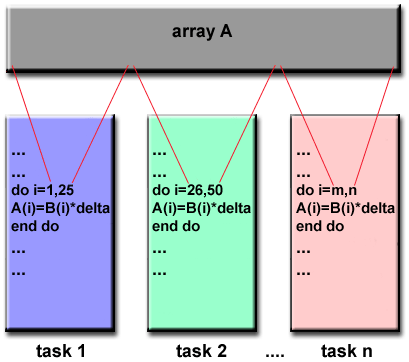
\includegraphics[width=\textwidth]{pictures/data-parallelism}
\centering{
Data parallelism
} \\
Example: MPI (Message passing interface)
\end{minipage}~% ------- "~"  add space between figure -> ~ \quad \qquad
\begin{minipage}[t]{0.30\textwidth}

\centering
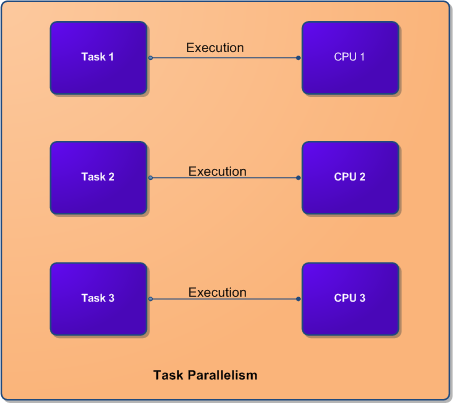
\includegraphics[width=\textwidth]{pictures/task-parallelism}
%\caption{Control parallelism}
\centering{
    Control parallelism
} \\
Example: HPF (High performance Fortran)
\end{minipage}

\end{figure}

\end{frame}

%--------------- frame ----------------

\begin{frame}
\frametitle{The aim of the \texttt{multifor}}

\begin{itemize}

\item In order to use more efficiently the resources of nowadays computers we have to work with appropriate tools.

\item The fact is that we already have lots of techniques to exhibit parallelism and optimize loops and wanted that not only compilers do that but programmers too.

\end{itemize}

\end{frame}

%-------------------- frame ----------------

\begin{frame}
\frametitle{Helping programmers}

\begin{itemize}

\item The programmer has only to worry about parallelizing and optimizing the code.
\item The \texttt{multifor} is only a control structure to simplify the implementation.
\item You can mix loops of different execution frequency and different starting point.

\end{itemize}

\end{frame}

%------------ frame ------------------

\begin{frame}
\frametitle{An incremental work}

The \texttt{multifor} will start by extending the C for structure. In the same way OpenMP is an extension to C/C++ and Fortran.\newline
In opposition we have the definition of new parallel languages like X10. \newline \newline
\begin{tabular}[l]{|p{0.48\textwidth}|p{0.48\textwidth}|}
\hline
\texttt{Multifor} & New parallel language \\
\hline
\color{green}{
    Is an extension of the well known for loop.\newline
    Can be implemented in existing languages.
}
&{
\color{green}{
Is implemented for parallel programming.
}
\color{red}{
\newline{}The programmer need to learn a new language and they often do not want.
}
}
\\
\hline
\end{tabular}

\end{frame}

%--------------- frame------------------

\subsection{Syntax and semantics reminding}

\begin{frame}
\frametitle{Syntax}

\small{ $\begin{array}{l}
    \bf{multifor}(int~{\color{red}i_0{=}0}, {\color{blue}i_1{=}0};
            {\color{red}i_0{<}6}, {\color{blue}i_1{<}3};
            {\color{red}i_0}++, {\color{blue}i_1}++;
            {\color{red}1}, {\color{blue}2};
            {\color{red}0}, {\color{blue}1})\{
    \\
        \quad{}\bf{multifor}(int~{\color{red}j_0{=}0}, {\color{blue}j_1{=}0};
                {\color{red}j_0{<}6}, {\color{blue}j_1{<}3};
                {\color{red}j_0}++, {\color{blue}j_1}++;
                {\color{red}1}, {\color{blue}2};
                {\color{red}0}, {\color{blue}2})\{
    \\
        \qquad{}{\color{red}0:\{ statement[i_0][j_0]\ldots \}}
    \\
        \qquad{}{\color{blue}1:\{ statement[i_1][j_1]\ldots \}}
    \\
        \quad{}\}
\\
    \}
\end{array}$
}

\centering{
    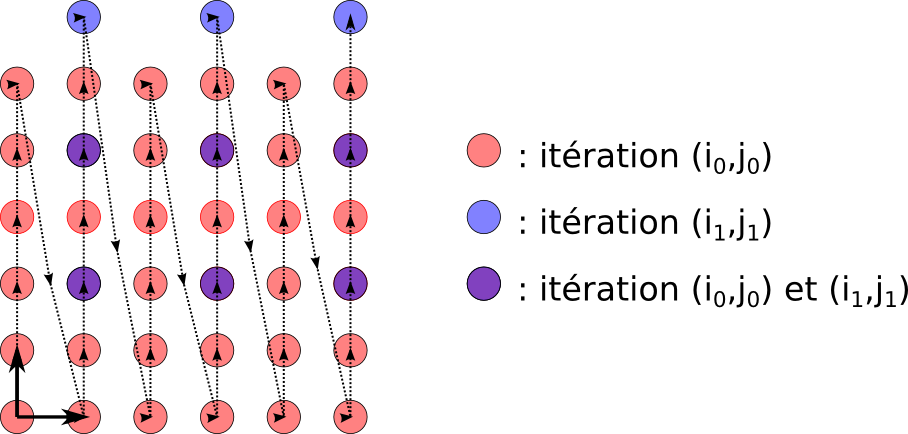
\includegraphics[height=3.5cm]{pictures/referential_domain}
}

\end{frame}

%-------------- frame -------------------

\section{From for to \texttt{multifor}}
\subsection{The game of life}

\begin{frame}
\frametitle{Game of life rules}

Rules:
\begin{itemize}
\item If a cell has exactly 3 neighbours it live the next time step.
\item If a cell has exactly 2 neighbours it states is unchanged.
\item Otherwise the cell dies.
\end{itemize}

\end{frame}

%------------- frame -------------

\begin{frame}
\frametitle{The game of life code}

{$\begin{array}{l}

    int~t[N][N]; \\
        int~temp[N-2][N-2]; \\ \\
        \textbf{void} calc ()\{ \\
        ~\textbf{{\color{red}for}}~(int~i=1; i<N-1; i++) \\
        \quad{}\textbf{{\color{red}for}}~(int~j=1; j<N-1; j++)\{ \\
        \qquad{}temp[{\color{green}i-1}][{\color{green}j-1}]=\\
        \qquad{}game\_of\_life(t[{\color{cyan}i}][{\color{cyan}j}],t[{\color{cyan}i-1}][{\color{cyan}j}],t[{\color{cyan}i-1}][{\color{cyan}j-1}],t[{\color{cyan}i-1}][{\color{cyan}j+1}],\\
                \qquad{}[{\color{cyan}i}][{\color{cyan}j-1}],[{\color{cyan}i}][{\color{cyan}j+1}],[{\color{cyan}i+1}][{\color{cyan}j-1}],[{\color{cyan}i+1}][{\color{cyan}j}],[{\color{cyan}i+1}][{\color{cyan}j+1}]); \\
        \quad{}\}\\
        ~\textbf{{\color{blue}for}}~(int~i=1; i<N-1; i++) \\
        \quad{}\textbf{{\color{blue}for}}~(int~j=1; j<N-1; j++)\{ \\
        \qquad{}t[i][j]=temp[i-1][j-1]; \\
        \quad{}\} \\
        \}



\end{array}$
}

\end{frame}

%---------- frame -------------

\begin{frame}
\frametitle{The game of life iteration domain}

\centering{
\includegraphics{pictures/gameoflife}
}

\end{frame}

%------------------- frame -------------------

\begin{frame}
\frametitle{The same algorithm written with a \texttt{mulifor}}

{$\begin{array}{l}

    void~calc\_multifor ()\{ \\
        ~multifor({\color{red}i=1}, {\color{blue}i2=1}; {\color{red}i<N-1}, {\color{blue}i2<N-1}; {\color{red}i++}, {\color{blue}i2++};{\color{red} 1}, {\color{blue}1}; {\color{red}0}, {\color{blue}3})\{ \\
            \quad{}multifor({\color{red}j=1}, {\color{blue}j2=1}; {\color{red}j<N-1}, {\color{blue}j2<N-1}; {\color{red}j++}, {\color{blue}j2++}; {\color{red}1}, {\color{blue}1}; {\color{red}0}, {\color{blue}0})\{ \\
\qquad{}0:\{\\
\qquad{}~~{\color{red}temp[i-1][j-1]=} \\
\qquad{}~~{\color{red}game\_of\_life(t[i][j],t[i-1][j],t[i-1][j-1],t[i-1][j+1],} \\
\qquad{}~~{\color{red}[i][j-1],[i][j+1],[i+1][j-1],[i+1][j],[i+1][j+1]);} \\
\qquad{}\} \\
\qquad{}1:~~{\color{blue}t[i2][j2]=temp[i2-1][j2-1];} \\
           \quad{}\} \\
        ~\} \\
    \} \\


    \end{array}$
}

\end{frame}

%--------------- frame ----------------

\begin{frame}
\frametitle{Using ISL}

After expressing the loop in the referential domain we got:
\begin{equation}
\scriptsize{D1 := [N]\rightarrow{}[i,j,i,j]:1<=i<N-1, 1<=j<N-1}
\end{equation}
\begin{equation}
\scriptsize{D2 := [N]\rightarrow{}[i2',j2,i2,j2] : i2'=i2+3, 1<=i2<N-1, 1<=j2<N-1}
\end{equation}
We give this two equations to ISL and we got the loops.

\end{frame}

%------------ frame ------ 

\begin{frame}
\frametitle{The obtained loops}

{$\begin{array}{l}
for(int~i=1; i<N-1; i++)\{ \\
~for(int~j=1; j<N-1; j++)\{ \\
\quad{}compute(i,j); \\
\quad{}if(i>=4)\{ \\
\qquad{}copie(i-3,j); \\
\quad{}\} \\
~\} \\
\} \\
for(int~i=\max(4, N-1); i<=N+1; i++)\{ \\
~for(j=1; j<N-1; j++)\{ \\
\quad{}copie(i-3,j); \\
~\} \\
\} \\
\end{array}$
}

\end{frame}

%------- frame -------

\subsection{Two matrix multiplication}

\begin{frame}
\frametitle{The algorithm}

{$\begin{array}{l}
D= alpha\times{}A\times{}B\times{}C + beta\times{}D \\ \\
for (int~i = 0; i < I; i++) \\
~for (int~j = 0; j < J; j++)\{ \\
\quad{}tmp[i][j] = 0; \\
\quad{}for (k = 0; k < K; ++k) \\
\qquad{}tmp[i][j] += alpha * A[i][k] * B[k][j]; \\
~\} \\
for (int~i = 0; i < I; i++) \\
~for (int~j = 0; j < L; j++)\{ \\
\quad{}D[i][j] *= beta; \\
\quad{}for (k = 0; k < J; ++k) \\
\qquad{}D[i][j] += tmp[i][k] * C[k][j]; \\
~\}

\end{array}$
}
\end{frame}

% ------------- frame ------------

\begin{frame}
\frametitle{Dependency resolution}

I used Philippe's api to display dependencies in order to write the \texttt{multifor} \\
\centering
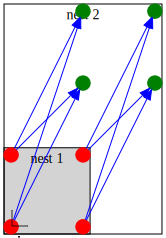
\includegraphics[height=4cm]{pictures/2mm}

\end{frame}

%---------- frame ------------

\begin{frame}
\frametitle{Nested \texttt{multifor}}

{\footnotesize$\begin{array}{l}
multifor(i1=0, i2=0; i1< I, i2< I; i1++, i2++; 1, 1; 0, {\color{red}1})\{ \\
~multifor(j1=0, j2=0; j1< J, j2< L; j1++, j2++; 1, 1; 0, 0)\{ \\
\quad{}0:\{ \\
\qquad{}tmp[i1][j1]=0; \\
\quad{}\} \\
\quad{}1:\{ \\
\qquad{}D[i2][j2]*=beta; \\
\quad{}\} \\
\quad{}multifor(k1=0, k2=0; k1< K, k2< J; k1++, k2++; 1, 1; 0, 0)\{ \\
\qquad{}0:\{ \\
\qquad{}~~tmp[i1][j1]+=alpha* A[i1][k1]* B[k1][j1]; \\
\qquad{}\} \\
\qquad{}1:\{ \\
\qquad{}~~D[i2][j2]+= tmp[i2][k2] * C[k2][j2]; \\
\qquad{}\} \\
\quad{}\} \\
~\} \\
\}
\end{array}$
}

\end{frame}

%--------- frame ---------

\begin{frame}
\frametitle{Referential domain}

\centering{
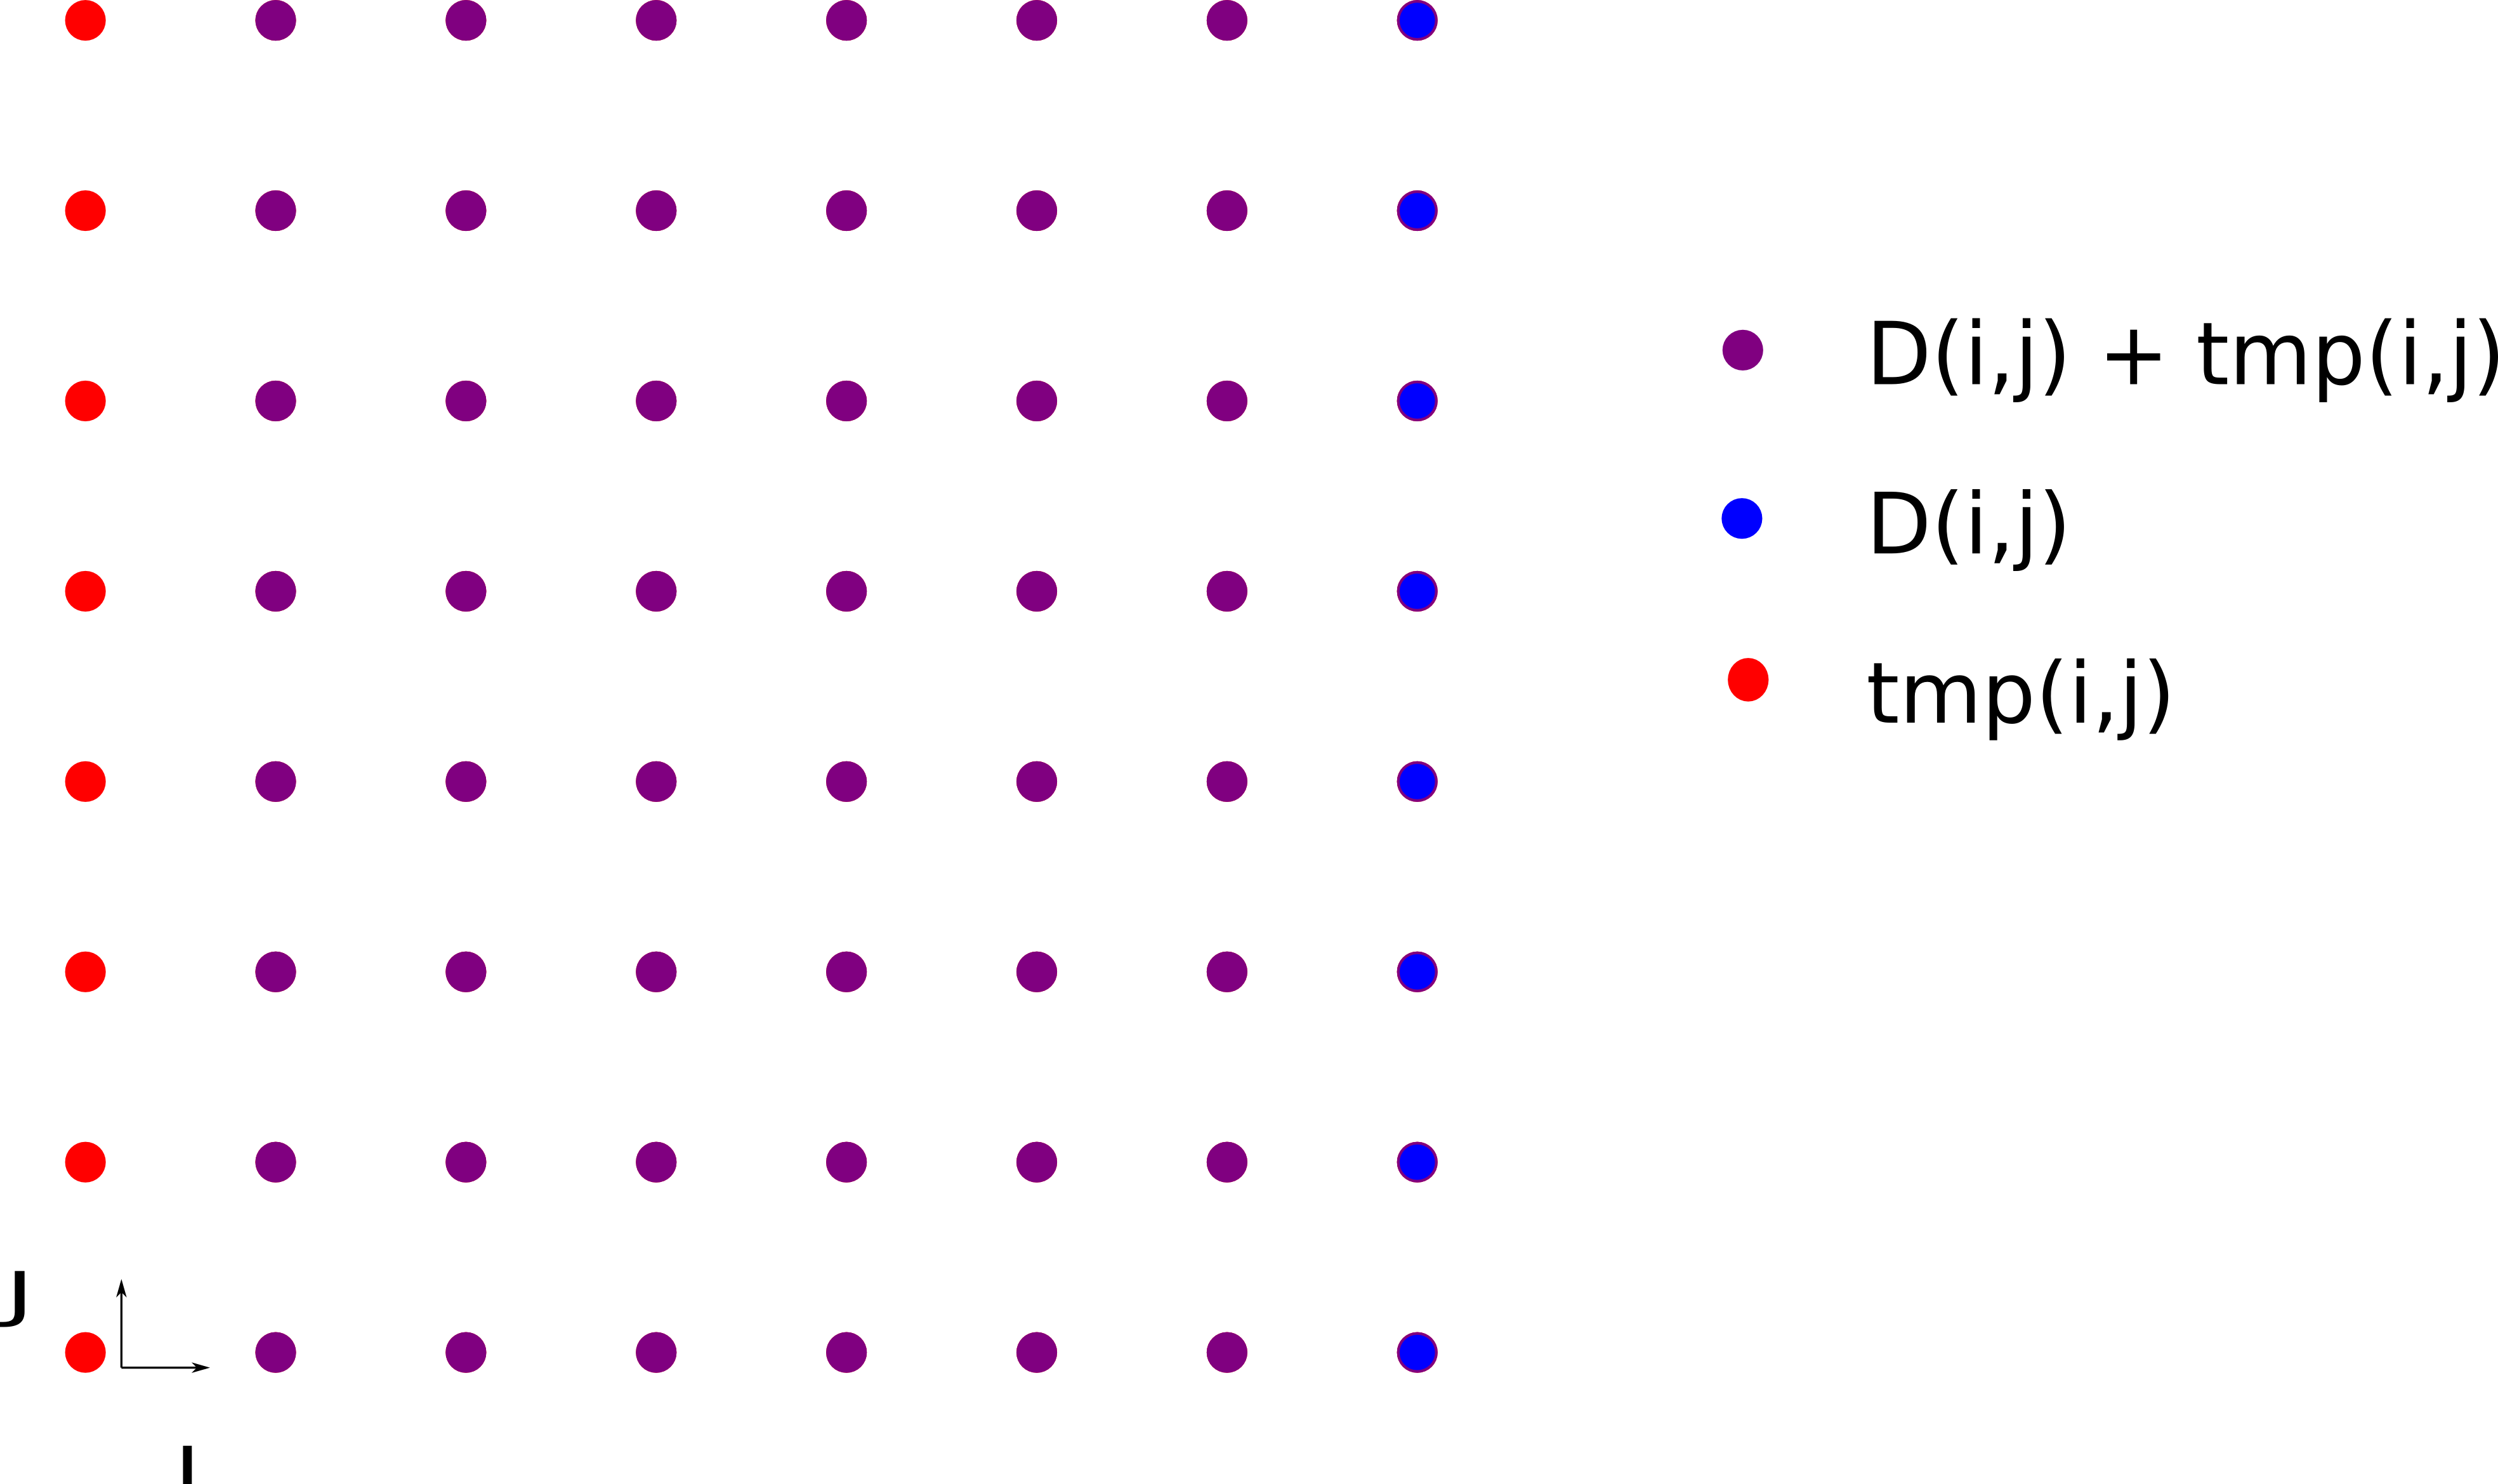
\includegraphics[height=5cm]{pictures/2mmdomain}
}

\end{frame}

%------------ frame ------------

\subsection{Tree matrix multiplication}

\begin{frame}
\frametitle{Algorithm}

\only<1>{
$E = A\times{}B $
$\begin{array}{l}
for (i = 0; i < I; i++) \\
~for (j = 0; j < I; j++)\{ \\
\quad{}E[i][j] = 0; \\
\quad{}for (k = 0; k < I; ++k) \\
\qquad{}E[i][j] += A[i][k] * B[k][j]; \\
~\}
\end{array}$
}
\only<2>{
$F = C\times{}D $
$\begin{array}{l}
for (i = 0; i < I; i++) \\
~for (j = 0; j < I; j++)\{ \\
\quad{}F[i][j] = 0; \\
\quad{}for (k = 0; k < I; ++k) \\
\qquad{}F[i][j] += C[i][k] * D[k][j]; \\
~\}
\end{array}$
}
\only<3>{
$G = E\times{}F$
$\begin{array}{l}
for (i = 0; i < I; i++) \\
~for (j = 0; j < I; j++)\{ \\
\quad{}G[i][j] = 0; \\
\quad{}for (k = 0; k < I; ++k) \\
\qquad{}G[i][j] += E[i][k] * F[k][j]; \\
~\}
\end{array}$
}

\end{frame}

%--------- frame ---------

\begin{frame}
\frametitle{Dependencies}

\only<1>{
    How E is calculated \newline{} \\
    \centering{
    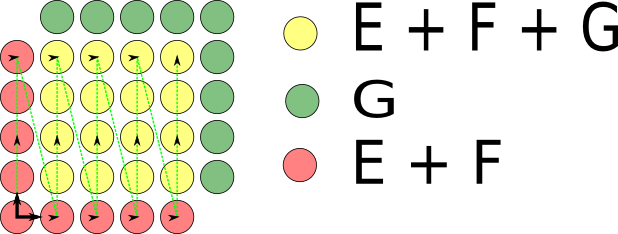
\includegraphics[height=2.5cm]{pictures/3mmdomain1}
    }
}

\only<2>{
How F is calculated \newline{} \\
\centering{
\includegraphics[height=2.5cm]{pictures/3mmdomain2}
}
}

\only<3>{
How G is calculated \\
The order of the computation is not important within the ``V'' structure \\
\centering{
\includegraphics[height=2.5cm]{pictures/3mmdomain3}
}
}

\end{frame}

%-------- frame --------

\begin{frame}
\frametitle{Base change}

Whith two loop nest you can express the \texttt{multifor} like this:
\newline{} \newline{}
\begin{math}
\begin{cases}
x'=gx+o \\
y'=g_x y + o_x + g'x+o'
\end{cases}
\end{math} \newline \newline
But by making an \begin{math}\frac{\pi}{4}\end{math} rotation we get this expression \newline \newline
\begin{math}
\begin{cases}
x'= x+y \\
y'=y-x
\end{cases}
\end{math}\newline \newline 
So it is impossible to express this rotation with the \texttt{multifor} semantics for now

\end{frame}

%------- frame --------

\begin{frame}
\frametitle{\texttt{Multifor} representation}
\only<1>{
So I made a function to calculate the ``V'' structure in function of a given row \newline{} \\
\footnotesize{$\begin{array}{l}
void~calculation(int~i, int~I, double *G,double *E, double*F,\\
~int~bool)\{ \\
\quad{}for(int~ibis=i, jbis=-i; jbis<-i+I; ibis++, jbis++)\{ \\
\qquad{}int~ibase=(ibis-jbis)/2, jbase=(ibis+jbis)/2; \\
\qquad{}if( (bool~\&\&~jbis<=0)~||~(!bool~\&\&~jbis>0))\{ \\
\qquad{}~~G[ibase][jbase]=0; \\
\qquad{}~~for(int k=0; k<I; k++)\{ \\
\qquad{}\quad{}~~G[ibase][jbase]+=E[ibase][k]* F[k][jbase]; \\
\qquad{}~~\} \\
\qquad{}\}\\
\quad{}\}\\
~\}\\
\end{array}$
}
}
\only<2>{
This is the multifor related \newline{} \\
\footnotesize{$\begin{array}{l}
multifor(i1=0, i2=0, {\color{red}i3=0}, {\color{blue}i4=0}; i1<I, i2<I, {\color{red}i3<I}, {\color{blue}i4<I};\\
~~~i1++, i2++, {\color{red}i3++}, {\color{blue}i4++}; 1, 1, {\color{red}1}, {\color{blue}1}; 0, 0, {\color{red}-1}, {\color{blue}1})\{ \\
~2: calculation(i3,I,G,E,F,{\color{red}0});\\
~3: calculation(i4,I,G,E,F,{\color{blue}1});\\
~multifor(j1=0, j2=0; j1 < I, j2<I; j1++, j2++;1, 1; 0, 0)\{ \\
\quad{}0: E[i1][j1]=0; \\
\quad{}1: F[j2][i2]=0;\\
\quad{}multifor(k1=0, k2=0; k1 < I, k2<I; k1++, k2++; 1, 1; 0, 0)\{ \\
\qquad{}0: E[i1][j1]+=A[i1][k1]*B[k1][j1]; \\
\qquad{}1: F[j2][i2]+=C[j2][k2]*D[k2][i2]; \\
\quad{}\}\\
~\}\\
\}\\
\end{array}$
}
}


\end{frame}

%------------ frame -----------
\subsection{Floyd-Warshall}

\begin{frame}
\frametitle{The algorithm}
This algorithm repeats N times the same job on a NxN matrix\newline \\
{$\begin{array}{l}
for (k = 0; k < N; k++)\{ \\
~for(i = 0; i < N; i++) \\
\quad{}for (j = 0; j < N; j++) \\
\qquad{}path[i][j] = path[i][j] < path[i][k] + path[k][j]~? \\
\qquad{}path[i][j] : path[i][k] + path[k][j]; \\
\} \\
\end{array}$
}

\end{frame}

\begin{frame}
\frametitle{Referential domain}

\centering
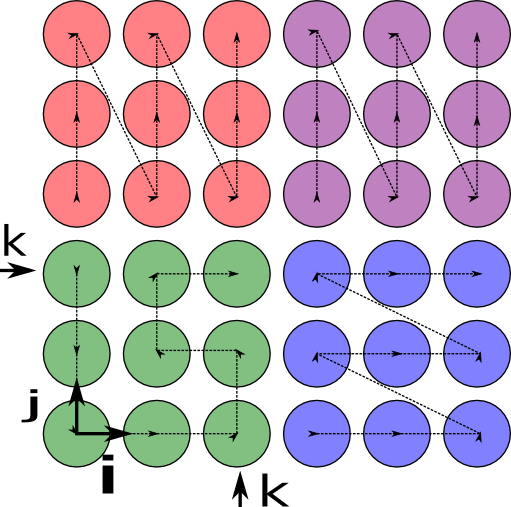
\includegraphics[height=4cm]{pictures/floyd-warshall-domain}

\end{frame}

%------------ frame ---------

\begin{frame}
\frametitle{\texttt{Multifor} algorithm}
\scriptsize{$\begin{array}{l}
for(int~k=0; k< N; k++)\{ \\
~multifor(i1=0,i2=0,j3=0; i1<k+1, i2<k+1, j3<k+1;\\
~~i1++,i2++,j3++; 1,1,1; 0,1,1)\{ \\
\quad{}0: mult1(i1, path, k); \\
\quad{}1: mult2(i2,path,k); \\
\quad{}2: mult3(j3,path,n,k); \\
~\} \\
~for(int i=k+1; i<n;i++)\{ \\
\quad{}for(int j=k+1;j<n;j++)\{ \\
\qquad{}path[i][j] = path[i][j] < path[i][k] + path[k][j] ? path[i][j] : path[i][k] + path[k][j]; \\
\quad{}\} \\
~\} \\
\}
\end{array}$
}
\end{frame}

%---------------- frame -------------

\section{Benchmark}

\begin{frame}
\frametitle{Two matrix}
\centering
%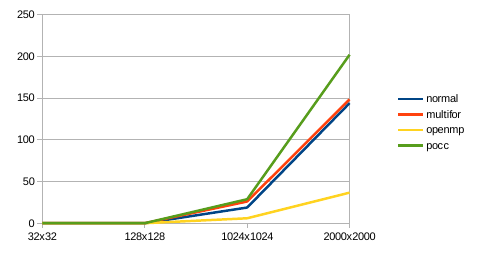
\includegraphics[height=5cm]{pictures/2mmbench}

\end{frame}

%----------- frame -----------

\begin{frame}
\frametitle{Tree matrix}
\centering
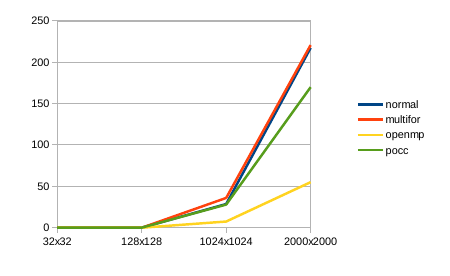
\includegraphics[height=5cm]{pictures/3mmbench}
\end{frame}

% ---------- frame ---------

\subsection{Tools used}

\begin{frame}
\frametitle{Tools}

The polybench can be found on http://www.cse.ohio-state.edu/$\sim$pouchet/software/polybench/ and belongs to Louis-Noel Pouchet. The documentation is included in the archive. \\
ISL was used with an online interface that you can found here: http://www.cs.kuleuven.be/cgi-bin/dtai/barvinok.cgi \\
IBB uses C code as input which can include a multifor and produces a C code that can be compiled. For more information ask Imèn Fassi at fassi.imen@gmail.com \\
ClooG is used in both IBB and ISL. For more informations please visit the web site www.cloog.org/ \\
POCC is a compiler collection for C code to optimized C code. Please visit www.cs.ucla.edu/$\sim$pouchet/software/pocc/ for more informations. \\

\end{frame}

\end{document}
